\begin{figure}[htbp]
\centering
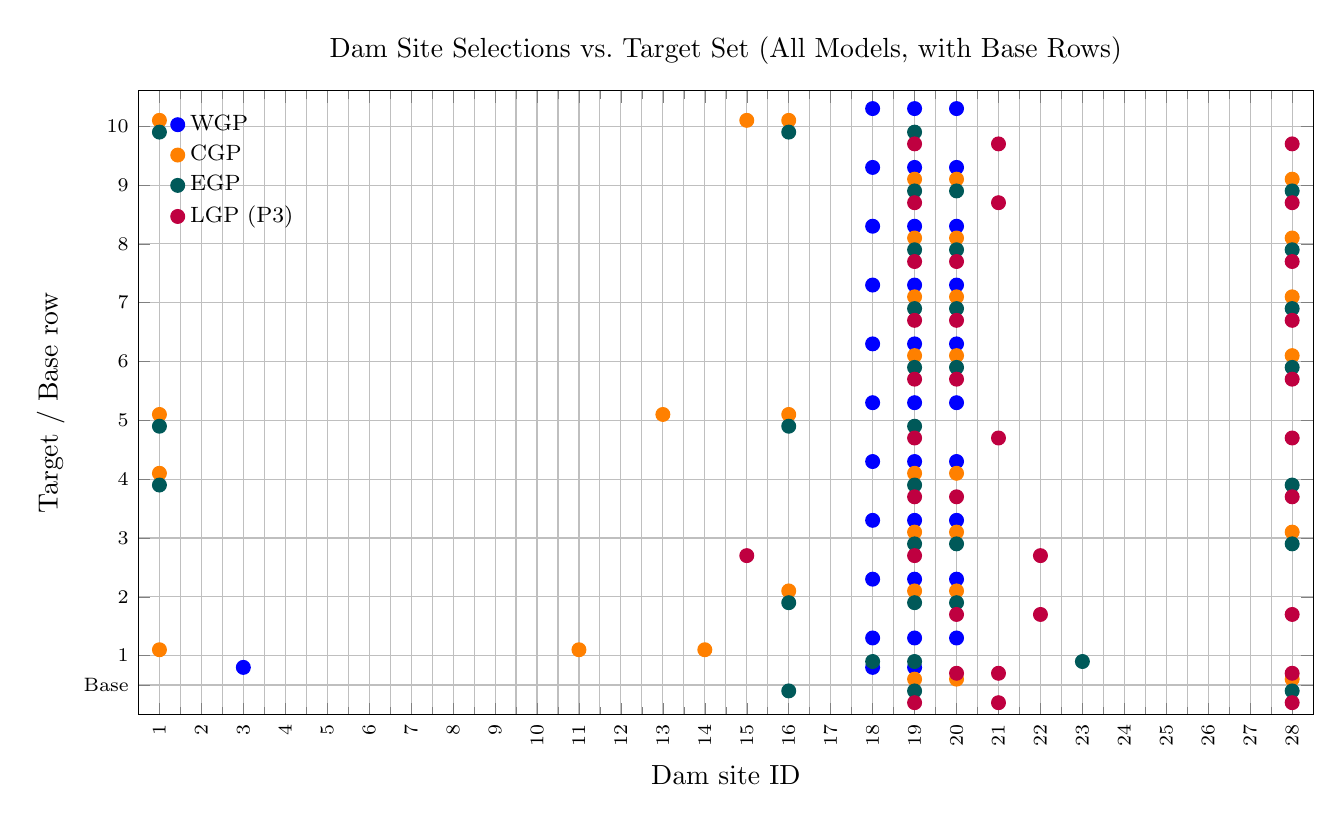
\begin{tikzpicture}
  \begin{axis}[
    title={Dam Site Selections vs.\ Target Set (All Models, with Base Rows)},
    xlabel={Dam site ID},
    ylabel={Target / Base row},
    xmin=0.5, xmax=28.5,
    ymin=0.0, ymax=10.6,
    xtick={1,2,...,28},
    ytick={0.5,1,2,3,4,5,6,7,8,9,10},
    yticklabels={Base,1,2,3,4,5,6,7,8,9,10},
    x tick label style={font=\scriptsize, rotate=90, anchor=east},
    y tick label style={font=\scriptsize},
    width=16.5cm, height=9.5cm,
    grid=both, minor tick num=1,
    legend style={at={(0.02,0.98)}, anchor=north west, draw=none, fill=none, font=\footnotesize},
    legend cell align=left
  ]

  

  % ---- Model row offsets (constant across all targets) ----
  % Base anchor row at y=0.5
  % WGP: +0.30 ; CGP: +0.10 ; EGP: -0.10 ; LGP: -0.30
  % For target set t, rows are: t+0.30 (WGP), t+0.10 (CGP), t-0.10 (EGP), t-0.30 (LGP)

  % ===================== WGP =====================
  \addplot+[only marks, mark=*, mark options={fill=blue, draw=blue}, mark size=2.5pt]
    coordinates
    % --- Base (WGP base selected: 18,19,3) at y=0.5+0.30=0.80
    {(3,0.80) (18,0.80) (19,0.80)
    % --- Target sets (always 18,19,20)
     (18,1.30) (19,1.30) (20,1.30)
     (18,2.30) (19,2.30) (20,2.30)
     (18,3.30) (19,3.30) (20,3.30)
     (18,4.30) (19,4.30) (20,4.30)
     (18,5.30) (19,5.30) (20,5.30)
     (18,6.30) (19,6.30) (20,6.30)
     (18,7.30) (19,7.30) (20,7.30)
     (18,8.30) (19,8.30) (20,8.30)
     (18,9.30) (19,9.30) (20,9.30)
     (18,10.30) (19,10.30) (20,10.30)};
  \addlegendentry{WGP}

  % ===================== CGP =====================
  \addplot+[only marks, mark=*, mark options={fill=orange, draw=orange}, mark size=2.5pt]
    coordinates
    % --- Base (CGP base: 19,20,28) at y=0.5+0.10=0.60
    {(19,0.60) (20,0.60) (28,0.60)
    % --- Target set 1: 1,11,14
     (1,1.10) (11,1.10) (14,1.10)
    % --- 2: 16,19,20
     (16,2.10) (19,2.10) (20,2.10)
    % --- 3: 19,20,28
     (19,3.10) (20,3.10) (28,3.10)
    % --- 4: 1,19,20
     (1,4.10) (19,4.10) (20,4.10)
    % --- 5: 1,13,16
     (1,5.10) (13,5.10) (16,5.10)
    % --- 6: 19,20,28
     (19,6.10) (20,6.10) (28,6.10)
    % --- 7: 19,20,28
     (19,7.10) (20,7.10) (28,7.10)
    % --- 8: 19,20,28
     (19,8.10) (20,8.10) (28,8.10)
    % --- 9: 19,20,28
     (19,9.10) (20,9.10) (28,9.10)
    % --- 10: 1,15,16
     (1,10.10) (15,10.10) (16,10.10)};
  \addlegendentry{CGP}

  % ===================== EGP =====================
  \addplot+[only marks, mark=*, mark options={fill=teal!70!black, draw=teal!70!black}, mark size=2.5pt]
    coordinates
    % --- Base (EGP base: 16,19,28) at y=0.5-0.10=0.40
    {(16,0.40) (19,0.40) (28,0.40)
    % --- 1: 18,19,23
     (18,0.90) (19,0.90) (23,0.90)
    % --- 2: 16,19,20
     (16,1.90) (19,1.90) (20,1.90)
    % --- 3: 19,20,28
     (19,2.90) (20,2.90) (28,2.90)
    % --- 4: 1,19,28
     (1,3.90) (19,3.90) (28,3.90)
    % --- 5: 1,16,19
     (1,4.90) (16,4.90) (19,4.90)
    % --- 6: 19,20,28
     (19,5.90) (20,5.90) (28,5.90)
    % --- 7: 19,20,28
     (19,6.90) (20,6.90) (28,6.90)
    % --- 8: 19,20,28
     (19,7.90) (20,7.90) (28,7.90)
    % --- 9: 19,20,28
     (19,8.90) (20,8.90) (28,8.90)
    % --- 10: 1,16,19
     (1,9.90) (16,9.90) (19,9.90)};
  \addlegendentry{EGP}

  % ===================== LGP (Priority 3) =====================
  \addplot+[only marks, mark=*, mark options={fill=purple, draw=purple}, mark size=2.5pt]
    coordinates
    % --- Base (LGP base P3: 19,21,28) at y=0.5-0.30=0.20
    {(19,0.20) (21,0.20) (28,0.20)
    % --- 1: 20,21,28
     (20,0.70) (21,0.70) (28,0.70)
    % --- 2: 20,22,28
     (20,1.70) (22,1.70) (28,1.70)
    % --- 3: 15,19,22
     (15,2.70) (19,2.70) (22,2.70)
    % --- 4: 19,20,28
     (19,3.70) (20,3.70) (28,3.70)
    % --- 5: 19,21,28
     (19,4.70) (21,4.70) (28,4.70)
    % --- 6: 19,20,28
     (19,5.70) (20,5.70) (28,5.70)
    % --- 7: 19,20,28
     (19,6.70) (20,6.70) (28,6.70)
    % --- 8: 19,20,28
     (19,7.70) (20,7.70) (28,7.70)
    % --- 9: 19,21,28
     (19,8.70) (21,8.70) (28,8.70)
    % --- 10: 19,21,28
     (19,9.70) (21,9.70) (28,9.70)};
  \addlegendentry{LGP (P3)}

  % --- A small guide on offsets (optional)
  \node[anchor=west, font=\scriptsize, align=left] at (axis cs:28.6,10.4)
    {Offsets per target row: \\
     WGP: +0.30,\ CGP: +0.10,\\
     EGP: $-0.10$,\ LGP: $-0.30$.\\
     Base row anchored at 0.5.};
  \end{axis}
\end{tikzpicture}
\caption{Selected dam sites by model and target set (circles; slight vertical offsets prevent overlap). Base models included on the “Base” row.}
\label{fig:dam_selection_targets_all_models}
\end{figure}






